\documentclass{article}

\usepackage{graphicx}
\usepackage{tikz}
\usepackage{tikzsymbols}
\usetikzlibrary{calc,patterns,shapes.geometric}
\pagestyle{empty}
\usepackage[margin=0pt]{geometry}
\geometry{papersize={14in,12in}}

\def\centerarc[#1](#2)(#3:#4:#5){\draw[#1] ($(#2)+({#5*cos(#3)},{#5*sin(#3)})$) arc (#3:#4:#5);}

\begin{document}
	\begin{figure}
		\centering
		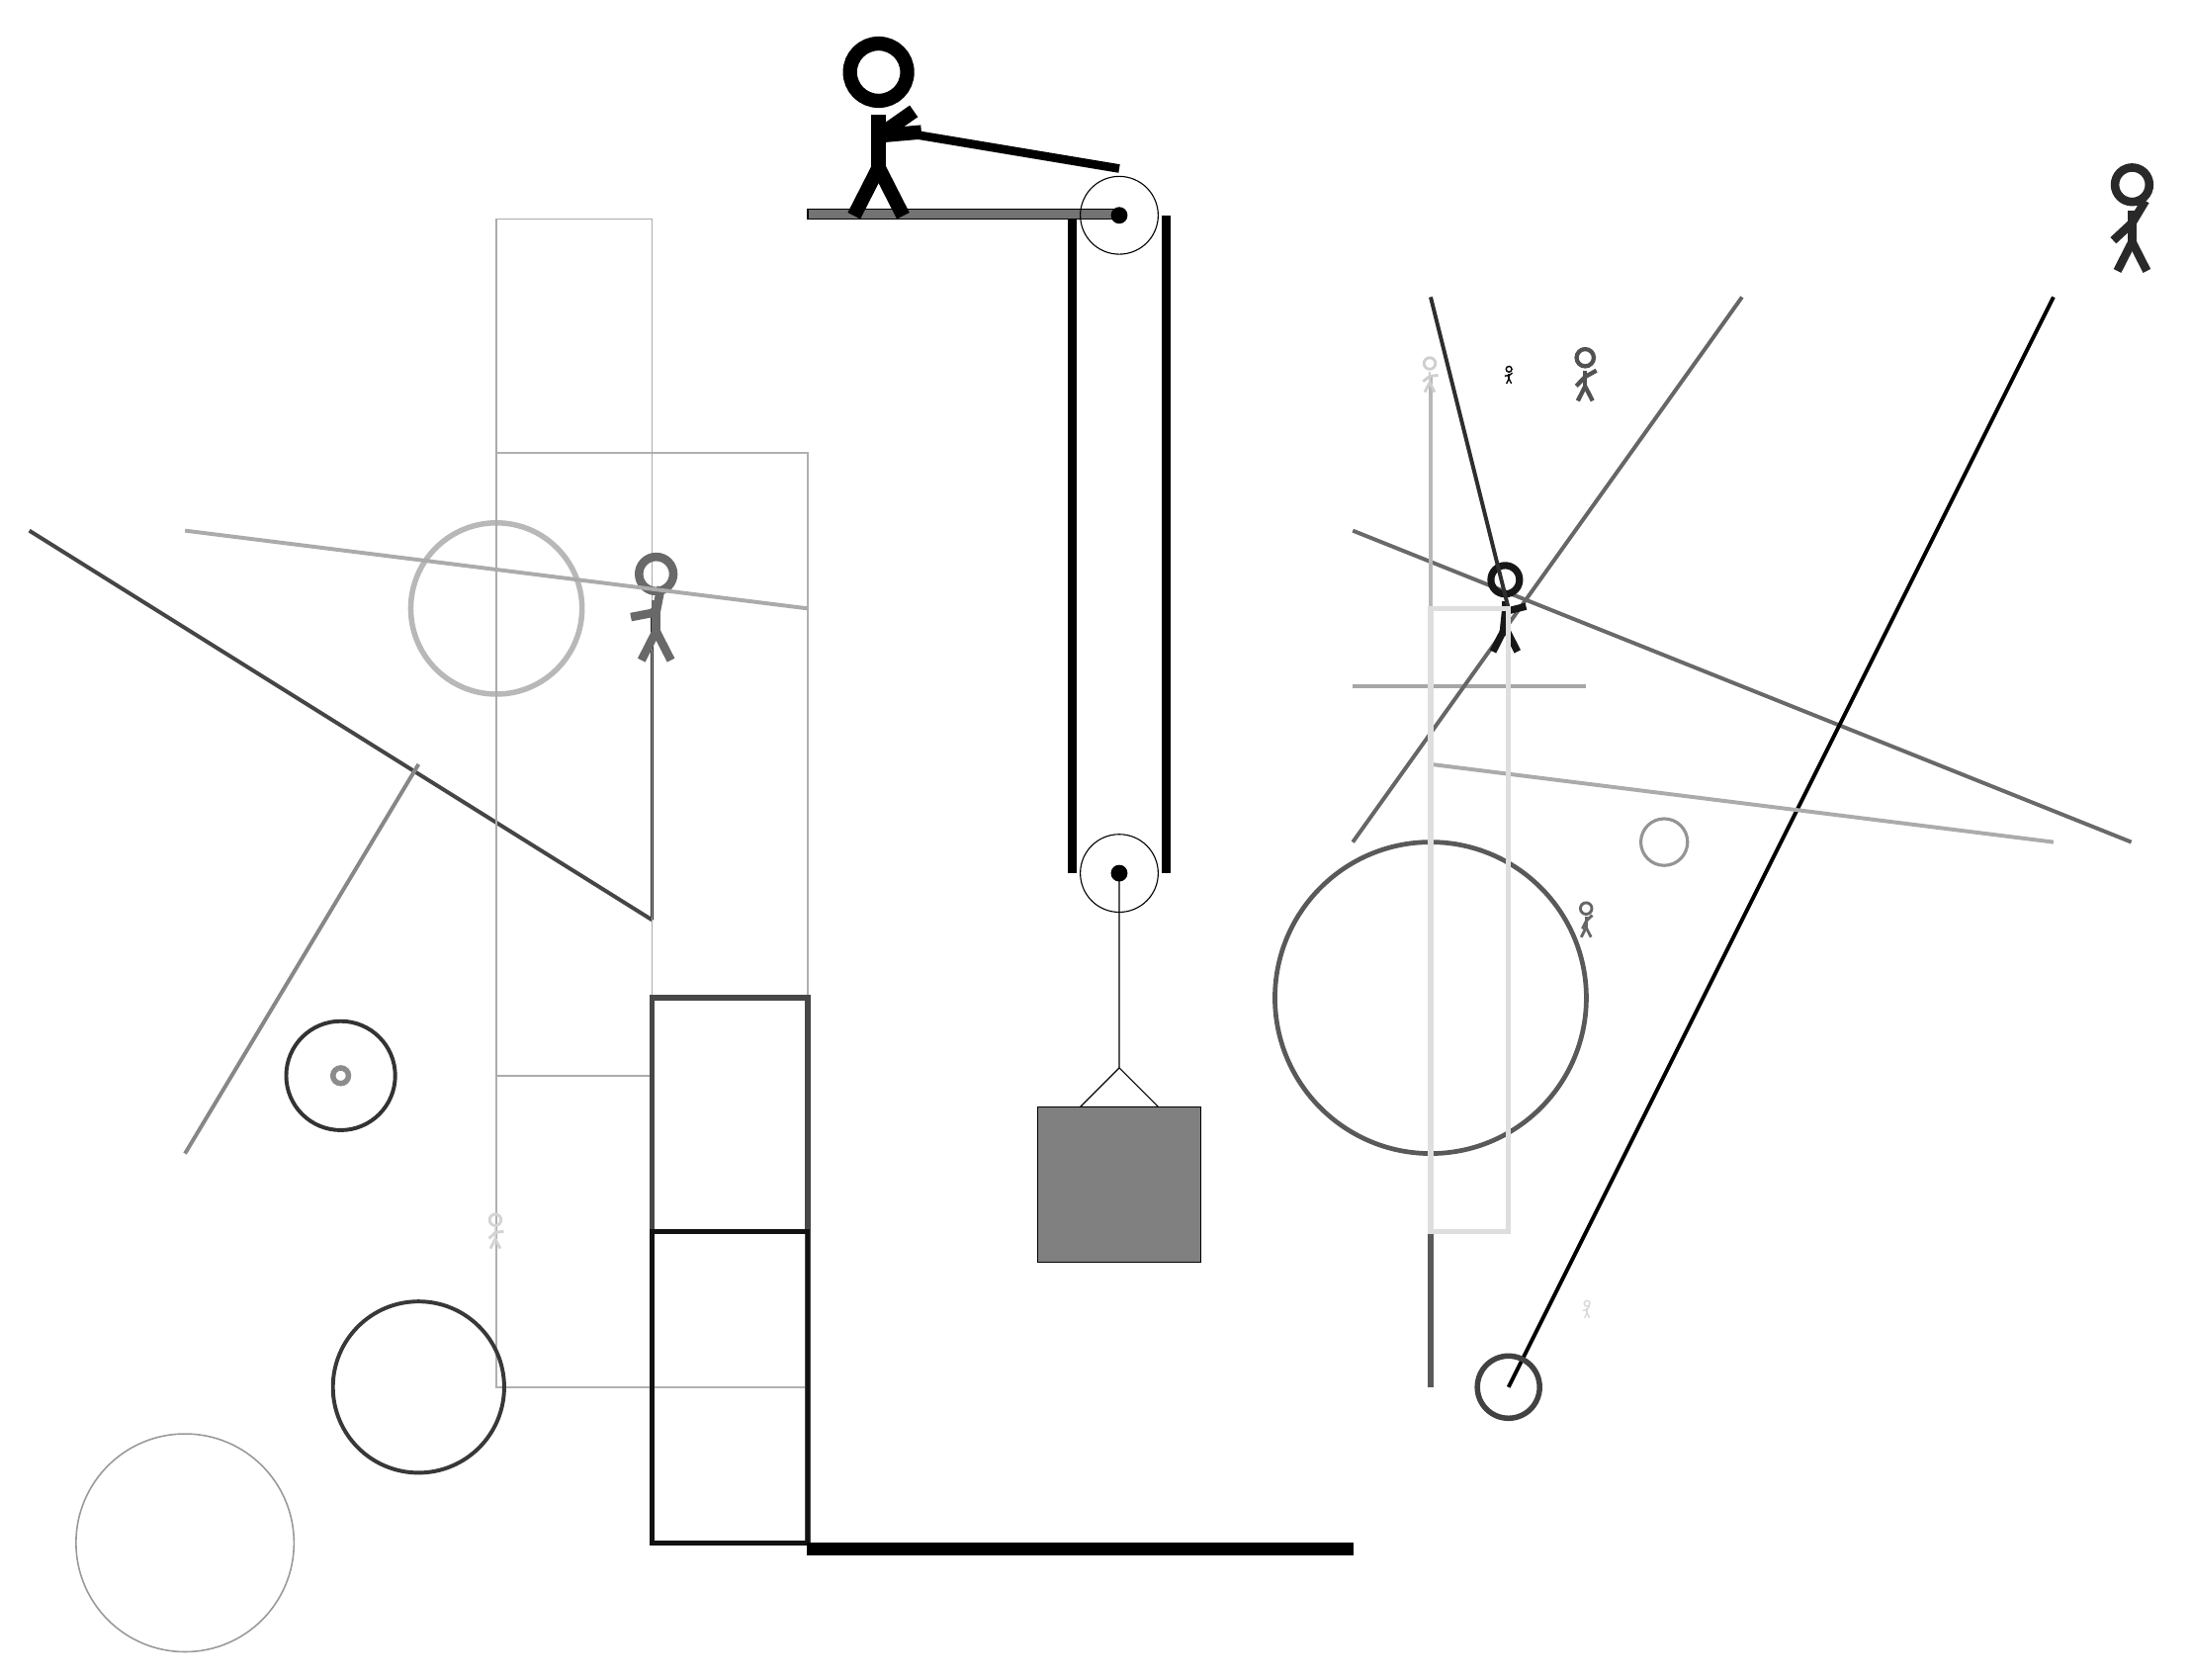
\begin{tikzpicture}
			%%%%% START %%%%%
			
			\draw[fill=black!55] (-2, 14) rectangle (2, 14.125);
			
			\draw (2, 5.6) circle (0.5);
			\draw[fill=black] (2, 5.6) circle (0.1);
			
			\draw (2, 14.05) circle (0.5);
			\draw[fill=black] (2, 14.05) circle (0.1);
			
			\draw (2, 5.6) -- (2, 3.1) -- (1.5, 2.6) -- (2.5, 2.6) -- (2, 3.1);
			\draw[fill=black!50] (0.95, 2.6) rectangle (3.05, 0.6);
			
			\draw [line width=0.7mm, color=black!28](-6, 9) circle (1.1);
			
			\draw[line width=0.3mm, color=black!86] (-4, 9) rectangle (-4, 5);
			\draw[line width=0.2mm, color=black!31] (-2, 11) rectangle (-6, -1);
			\node[line width=0.2mm, color=black!60] at (8, 5) {\Strichmaxerl[2][64][44]};
			
			\draw[line width=0.5mm, color=black!59](5, 10) -- (15, 6);
			\draw[line width=0.5mm, color=black!73](-4, 5) -- (-12, 10);
			\node[line width=0.5mm, color=black!17] at (-6, 1) {\Strichmaxerl[2][43][9]};
			
			\draw[line width=0.6mm, color=black!28] (6, 12) rectangle (6, 1);
			\draw[line width=0.2mm, color=black!33] (-4, 14) rectangle (-6, 3);
			\draw[line width=0.7mm, color=black!65] (6, 2) rectangle (6, -1);
			\draw[line width=0.7mm, color=black!72] (-2, -3) rectangle (-4, 4);
			
			\node[line width=0.4mm, color=black!68] at (8, 12) {\Strichmaxerl[3][46][29]};
			\draw[line width=0.5mm, color=black!100](7, -1) -- (14, 13);
			\draw[line width=0.6mm, color=black!93] (-2, 1) rectangle (-4, -3);
			\draw [line width=0.4mm, color=black!42](9, 6) circle (0.3);
			\node[line width=0.7mm, color=black!59] at (-4, 9) {\Strichmaxerl[6][11][79]};
			
			\draw [line width=0.7mm, color=black!74](7, -1) circle (0.4);
			\node[line width=0.2mm, color=black!84] at (15, 14) {\Strichmaxerl[6][43][59]};
			\draw [line width=0.5mm, color=black!78](-7, -1) circle (1.1);
			\node[line width=0.7mm, color=black!97] at (7, 12) {\Strichmaxerl[1][4][38]};
			\node[line width=0.4mm, color=black!15] at (8, 0) {\Strichmaxerl[1][9][61]};
			
			\draw [line width=0.2mm, color=black!40](-10, -3) circle (1.4);
			\draw[line width=0.5mm, color=black!33](6, 7) -- (14, 6);
			\draw [line width=0.6mm, color=black!65](6, 4) circle (2.0);
			\draw[line width=0.5mm, color=black!35](8, 8) -- (5, 8);
			\draw[line width=0.5mm, color=black!33](-2, 9) -- (-10, 10);
			\draw[line width=0.5mm, color=black!47](-7, 7) -- (-10, 2);
			\draw[line width=0.7mm, color=black!90] (6, 1) rectangle (7, 1);
			
			\draw[line width=0.5mm, color=black!60](5, 6) -- (10, 13);
			\draw [line width=0.7mm, color=black!45](-8, 3) circle (0.1);
			\node[line width=0.5mm, color=black!91] at (7, 9) {\Strichmaxerl[5][84][14]};
			
			\draw [line width=0.5mm, color=black!80](-8, 3) circle (0.7);
			\node[line width=0.4mm, color=black!19] at (6, 12) {\Strichmaxerl[2][39][6]};
			\draw[line width=0.5mm, color=black!82](7, 9) -- (6, 13);
			
			\draw[line width=0.7mm, color=black!13] (6, 9) rectangle (7, 1);
			
			\draw[line width=1.1mm] (1.4, 14) -- (1.4, 5.6);
			\centerarc[line width=1.1mm](2, 5.6)(180:360:0.6);
			\draw[line width=1.1mm](2.6, 5.6) -- (2.6, 14.05);
			\centerarc[line width=1.1mm](2, 14.05)(0:90:0.6);
			\draw[line width=1.1mm](2, 14.65) -- (-1, 15.15);
			
			\node at (-1, 15.15) {\Strichmaxerl[10][-175][35]};
			
			\draw[fill=black] (-2, -3) rectangle (5, -3.15);
			
			%%%%% END %%%%%
		\end{tikzpicture}
	\end{figure}	
\end{document}